\section{Design and Implementation }

\subsection{Hardware and Software}
This was run on a MacBook Pro computer with an intel processor using Icarus-Verilog.
Additionally, gtkwave software was used to monitor the modules input and outputs.

\subsection{TSC Design Overview}

The TSC (Trigger Surround Cache) has a 3 bit state register, a 32-bit timer,
a 32-bit triggered time (TRIGTM), and an internal ring buffer.
It is connected to the ADC (Analog-to-Digital Converter)
via a request (REQ), ready (RDY), and data (DAT) lines.
Additionally, the TSC can communicate with other HUB devices using triggered (TRD), Send Buffer (SBF),
serial data (SD), and completed data (CD) registers and wires.
Lastly, the TSC is connected to a external module that controls its clock (clk), start and reset lines.

\begin{figure}[H]
      \centering
      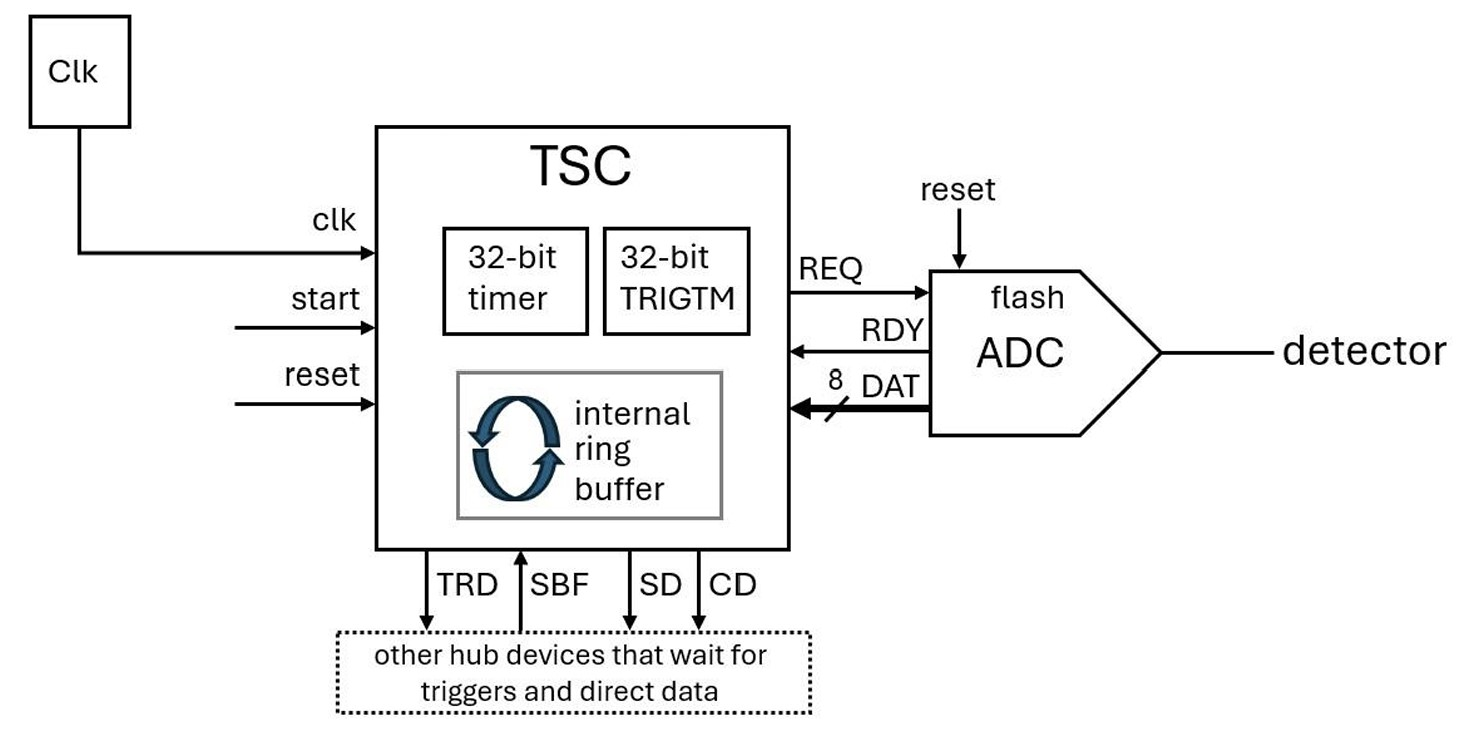
\includegraphics[width=0.8\columnwidth]{Figures/block_diagram_of_TSC}
      \caption{Block diagram of the TSC}
      \label{fig:block diagram of TSC}
\end{figure}

There is also an accompanying TSC\_tb test bench which is used to initiate and test the TSC module.
The test bench additionally simulates the HUB module.

\subsection{Clock (clk)}
A 250 MHz clock signal is set up on clk wire in the TS\_tb test bench.

\subsection{State Register}
The TSC module is run as a state machine where the state is a 3-bit register that has the following states:
\begin{itemize}
      \item \texttt{STOP} (0b000) :
            The state when the machine is powered on but has not been reset yet.
      \item \texttt{READY} (0b001) :
            The state where the module is awaiting a start command.
      \item \texttt{RUNNING} (0b010):
            The state entered after receiving a start command from \texttt{READY} or \texttt{IDLE}\@.
            In this state, the module increments the timer and writes adc values into the ring buffer.
      \item \texttt{TRIGGERED} (0b011):
            The state entered when a value read from the ADC is greater than the predetermined trigger value (TRIGVL).
            In this state, the module captures the next 16 adc values into the ring buffer
      \item \texttt{IDLE} (0b100);
            The state after the 16 adc values have been captured.
            This state signals to the HUB that the data is ready to be read, and the module awaits a start or SBF command.
      \item \texttt{SENDING} (0b101):
            This state is entered when it receives an SBF command from the \texttt{IDLE} state.
            It indicates that data is being sent on the SD line.
\end{itemize}

\subsection{Timer}
The timer is incremented on the rising edge of the clock.
When a trigger even occurs the timer is save in the TRIGTM register which is outputted to the test bench.
The timer is reset if a transition into a running state occurs.
To calculate the time of the trigger relative to the start command, the TRIGTM value is multiplied by the clock period (4 ps).

\subsection{Ring Buffer}
The ring buffer is used to store the values read by the ADC\@.
It is made up of 32 byte registers stored in an array called ring\_buffer.
The write pointer or tail is a 5-bit register (reg [4:0] write\_ptr).
Similarly, the read pointer or head is a 5-bit register as well (reg [4:0] read\_ptr) but is always one address ahead of the write pointer.

When adding new values to the ring buffer, the write pointer and read pointer are both incremented and then the value is written in the ring buffer at the address of the write pointer.
The write pointer is initially set to 5'b11111 such that the first write address is address 0.

When reading values from the ring buffer, the value at the read pointer is read and the read pointer is incremented; this is repeated until the read pointer is at the write pointer which indicates that all the values in the ring buffer have been read.

\subsection{How the TSC interfaces with the ADC}
The ADC is initialized in the TSC module, where the reset line is shared by both modules, the REQ line is controlled by the TSC module and the RDY and DAT lines are watched by TSC module.

When the TSC module requires a byte of data from the ADC module, it pulls the REQ line high, which causes the ADC module to output a byte of data on the DAT line and pull the RDY line high.
The TSC module responds to the rising edge of the RDY line, stores the byte on the DAT line, and finally drops the REQ line low.
The ADC module's data values come from a csv file of 256 randomly generated values.

Due to this being a simulation, all of the above would happen instantaneously, thus, artificial delay has been added to prevent the pulse from not showing on gktwave.
This can be seen in the two code sections \lref{lst:posedgerdy} and \lref{lst:clockrunning} below.
It should be noted that both code sections have safety measures in place.
\lref{lst:posedgerdy} checks that data was actually requested and \lref{lst:clockrunning} check that the data has been recorded and acknowledged before setting the REQ line back high.


\begin{lstlisting}[language=Verilog, caption={Verilog code for storing data and moving pointers on the posedge of RDY}, label={lst:posedgerdy}]
    always @(posedge RDY) begin
        if (REQ) begin
            #1 //delay so the pulse doesn't disappear on gktwave.
          
            //manage trigger_value ....

            //store data and move pointers around
            ring_buffer[++write_ptr] = adc_data;
            read_ptr++;

            adc_request = 0; //pull request down
        end
    end
\end{lstlisting}


\begin{lstlisting}[language=Verilog, caption={Verilog code for requesting data from the ADC on the posedge of the clock while in \texttt{RUNNING} state}, label={lst:clockrunning}]
    always @(posedge clk) begin
        case(state)
            `\texttt{RUNNING}: begin
                timer++;
                if (~ adc_request)
                    adc_request = 1; //request new adc value (handled with posedge adc_ready)
                end
            end

        //other cases

        endcase
    end
\end{lstlisting}

\subsection{Triggering}

The TSC module has a constant trigger value (TRIGVL) which is set in the TSC module but can also be overwritten in the test bench.
A trigger occurs when the TSC module is in the \texttt{RUNNING} state and the requested ADC DAT value is greater than the TRIGVL\@.
This causes the following to happen:

\begin{itemize}
      \item The TSC module transitions to the \texttt{TRIGGERED} state.
      \item The TRIGTM register is set to the current value of the timer.
      \item The register remaining\_values is set to 5'h10 (equivalent of decimal 16).
            This value will count down as the following 16 adc values are recorded into the ring buffer.
\end{itemize}

This Implementation is demonstrated in the code below.

\begin{lstlisting}[language=Verilog, caption={Code for triggering event in the TSC module}, label={lst:triggering}]
      //if it hasn't been triggered already, check for a valid trigger
      if (state != `TRIGERED) begin
            if (adc_data > TRIGVL) begin
                state = `TRIGERED;
                TRIGTM = timer; //capture time of trigger
                //set remaining adc values to 16 (handled by posedge clk)
                remaining_values = 5'h10;
            end
      end
\end{lstlisting}

When the TSC module is in the \texttt{TRIGGERED} state, the TSC does the following on the positive edge of the clock.

\begin{itemize}
    \item It increments the timer value because as per project brief the timer must only stop being incremented once the \texttt{IDLE} stat has been entered.
    \item It checks if remaining\_values is greater than zero, if so, it records the next byte from the adc into the ring buffer.
    \item If remaining\_values is zero, then all 16 bytes have been recoded and it transitions to the \texttt{IDLE} state, and pulls the TRD line to the HUB module high.
\end{itemize}

\begin{lstlisting}[language=Verilog, caption={Verilog code for recording 16 values after a trigger event}, label={lst:triggering2}]
    always @(posedge clk) begin
        case(state)
            `TRIGERED: begin
                timer++;
                //check that there are remaining values left to capture and decrement.
                if(remaining_values--)  begin
                    if (~ adc_request)
                        adc_request = 1; //request new adc value (handled with posedge adc_ready)
                    end else begin //all 16 values have been captured, wait for start or SBF command
                        state = `\texttt{IDLE};
                        TRD = 1'b1;
                    end
                end
            end

        //other cases

        endcase
    end
\end{lstlisting}

\subsection{Sending data to HUB devices}
To send data, the TSC module uses the following bit definitions for the current serial\_bit
when transmitting data via the SD line:

\begin{itemize}
      \item \texttt{WAIT\_BIT} (4'b1101): Wait for at least 1 positive edge of the clock for first start bit.
      \item \texttt{TRANSMISSION\_START\_BIT} (4'b1110): Use to pull the SD line low when the first byte is being sent.
      \item \texttt{END\_BIT} (4'b0111): Data byte only has bits 0--7, so reaching bit 7 means the byte has finished.
      \item \texttt{START\_BIT} (4'b1111): Start bit of the byte transmission
            The serial bit is always incremented BEFORE the bit is sent.
\end{itemize}

When the TSC module is in the \texttt{IDLE} state and the SBF line is pulled high, the TSC module will transition to the \texttt{SENDING} state.
During this transition, it will set SD high, CD low and serial\_bit = \texttt{WAIT\_BIT}.

If the TSC module in sending state and the serial\_bit = \texttt{WAIT\_BIT}, on the positive clock edge the serial\_bit will be set to equal \texttt{TRANSMISSION\_START\_BIT}.
This ensures that the TSC module will wait at least one full clock cycle before starting the fist byte of data.
Then on the next negative edge of the clock the start bit will be sent where the SD line will be set low and serial\_bit will be set to equal \texttt{START\_BIT}.

The TSC will then send the 8 bit data on the SD line on each negative edge of the clock using little endian format and incrementing serial\_bit each time.
After the 8 bits have been sent, the serial\_bit is set back to the \texttt{START\_BIT}, and the read pointer is incremented.
If the read pointer is at the write pointer, it means that the full ring buffer has been sent and the following occurs:

\begin{itemize}
    \item The read pointer is set back to in front of the write pointer.
    \item The state transitions into \texttt{READY}.
    \item The SD line is pulled low.
    \item The CD line is pulled high.
\end{itemize}



















